\documentclass[a4paper,12pt,oneside,openright]{abntex2}
%\documentclass[12pt]{abntex2}

% Pacotes básicos
\usepackage[brazil]{babel}
\usepackage[utf8]{inputenc}
\usepackage[T1]{fontenc}
\usepackage{microtype}
\usepackage{lmodern}
\usepackage{graphicx}
\usepackage{url}
\usepackage{amsmath,amssymb}
\usepackage{abntex2cite}
\usepackage{indentfirst}
\usepackage{graphicx}
\graphicspath{{images/}}
%\usepackage{parskip}
%\usepackage{fancyhdr}
%\usepackage{vmargin}
\setlength{\parindent}{0.75cm}

% =================================
% INSTRUÇÕES DO PROFESSOR
% [20%] Trabalho individual sobre as modalidades. Resumo* de 2-3 páginas por modalidade sobre as 5 modalidades: Ressonância Magnética, Medicina Nuclear, Raio-X, Ultra-som, OCT. A cada dia de atraso serão descontados 5% do valor máximo deste item. Depositar resumos no moodle. 
% ===================================


% Informações do trabalho
\title{Trabalho Modalidades de Imagens Médicas}
\author{Bruno Andreas S. C. V. Roma}
\local{São Paulo}
\data{2026}
%\theorientador{Sergio S. Furuie}

\makeatletter
\let\thetitle\@title
\let\theauthor\@author
\let\thedate\@date
\makeatother

%\pagestyle{fancy}
%\fancyhf{}
%\rhead{\theauthor}
%\lhead{\thetitle}
%\cfoot{\thepage}

\begin{document}

% Capa e folha de rosto
%\imprimircapa

\begin{titlepage}
	\centering
    \vspace*{0.2 cm}
    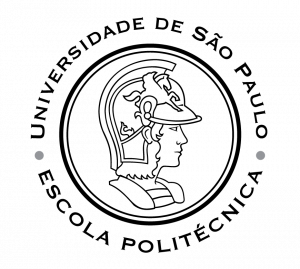
\includegraphics[scale = 1.25]{logo-poli-usp.png}\\[1.0 cm]	% University Logo
    %\textsc{\LARGE \newline\newline Escola Politécnica Da Universidade de São Paulo}\\[2.0 cm]	% University Name
    
	\textsc{\Large PTC5892 - Processamento de Imagens Médicas}\\[0.5 cm]				% Course Code
	
	\rule{\linewidth}{0.2 mm} \\[0.4 cm]
	{ \huge \bfseries \thetitle}\\
	\rule{\linewidth}{0.2 mm} \\[1.5 cm]
	
	\begin{minipage}{0.5\textwidth}
		\begin{flushleft} \large
			\emph{Professor:} \\ {Sergio S. Furuie}
			
			\end{flushleft}
			\end{minipage}~
			\begin{minipage}{0.4\textwidth}
            
			\begin{flushright} \large
			\emph{Aluno:} \\ {\theauthor}

		\end{flushright}
        
	\end{minipage}\\[2 cm]
	
	
    \thedate
    
    
    
	
\end{titlepage}

\pdfbookmark[0]{\contentsname}{toc}

\tableofcontents*

\cleardoublepage

\textual
\setcounter{page}{1}

\chapter{Raio-X e Tomografia Computadorizada}

\section{Fundamentos Físicos}

O diagnóstico por imagem fundamenta-se na interação da energia com a matéria biológica. No espectro eletromagnético, a energia é quantizada em fótons segundo a relação de Planck, $E = h \cdot f = h \cdot c / \lambda$, na qual $h$ representa a constante de Planck, $f$ a frequência, $c$ a velocidade da luz e $\lambda$ o comprimento de onda. Os raios-X ocupam a faixa de frequências superiores a $10^{16}\text{ Hz}$, com energias variando de $10^4\text{ a }10^5\text{ eV}$. Essa alta magnitude quântica confere aos raios-X caráter ionizante, capaz de ejetar elétrons orbitais de átomos, diferenciando-os de modalidades não ionizantes como a ressonância magnética nuclear e a ultrassonografia.

A produção de raios-X ocorre no interior de uma ampola composta de dois eletrodos submetidos a uma elevada diferença de potencial em quilovolts de pico ($\text{kVp}$). No cátodo, uma corrente em miliamperes ($\text{mA}$) aquece um filamento de tungstênio, liberando elétrons por emissão termoiônica. O gradiente de alta voltagem acelera esses elétrons em direção ao ânodo de tungstênio ($Z = 74$). Mais de noventa e cinco por cento da energia cinética incidente dissipa-se na forma de calor, demandando anodos giratórios e banhos de óleo dielétrico para refrigeração, enquanto a fração restante converte-se em fótons de raios-X por meio de dois processos simultâneos.

O primeiro mecanismo, a radiação de freamento (\textit{Bremsstrahlung}), decorre da desaceleração coulombiana que os elétrons experimentam ao passarem nas proximidades dos núcleos atômicos do alvo. A perda de energia cinética converte-se em um espectro contínuo de fótons de raios-X, cuja energia máxima equivale ao $\text{kVp}$ aplicado. O segundo mecanismo, a radiação característica, é estritamente quântico: um elétron incidente de alta energia colide de forma inelástica contra um elétron de uma camada interna do átomo do alvo (como a camada K), ejetando-o. A vacância é preenchida pela transição em cascata de elétrons de camadas mais externas (L ou M), com a liberação da diferença de energia de ligação sob a forma de fótons monoenergéticos característicos do material.

\section{Formação da Imagem por Transmissão}

A formação da imagem radiográfica assenta-se no princípio da transmissão e atenuação diferencial. Ao atravessar um meio biológico homogêneo, a atenuação de um feixe de raios-X segue a Lei de Lambert-Beer, expressa por:
\begin{equation}
I(x) = I_0 \cdot e^{-\mu \cdot x}
\end{equation}
em que $I_0$ é a intensidade incidente, $I(x)$ a intensidade transmitida após uma espessura $x$, e $\mu$ o coeficiente de atenuação linear. 

Como o coeficiente de atenuação linear $\mu$ varia de acordo com a densidade e a composição atômica de cada estrutura, estabelece-se o contraste radiológico característico dos tecidos humanos. O parênquima pulmonar aerado, com densidade mínima, atenua fracamente a radiação e projeta áreas escuras nas imagens. O tecido ósseo, rico em cálcio e fósforo com alta densidade, produz grande absorção fotoelétrica, resultando em sombras radiopacas (brancas) nas imagens. Músculo, água e gordura exibem coeficientes intermediários. Substâncias de alto número atômico, como o iodo ($Z = 53$) e o bário ($Z = 56$), são empregadas como meios de contraste artificiais por amplificarem o contraste radiológico. A radiação transmitida é capturada por detectores digitais planos (cintiladores acoplados a fotodiodos ou semicondutores diretos), enquanto grades antidifusoras absorvem a radiação espalhada para preservar a nitidez e o contraste geométrico da imagem.

\section{Princípios da Tomografia Computadorizada}

Embora indispensável, a radiografia convencional projeta estruturas tridimensionais sobrepostas em um plano bidimensional, dificultando a visualização de tais estruturas sobrepostas ou de baixo contraste. A tomografia computadorizada (TC) resolve essa restrição ao reconstruir matematicamente secções transversais a partir de projeções coletadas em múltiplos ângulos ao redor do paciente.

A base teórica da reconstrução tomográfica provém do Teorema de Radon (1917), segundo o qual uma distribuição espacial bidimensional de atenuação, $\mu(x, y)$, pode ser reconstruída a partir de um conjunto contínuo de suas integrais de linha (projeções angulares). O método analítico clássico empregado em sistemas clínicos é a Retroprojeção Filtrada (\textit{Filtered Backprojection} - $\text{FBP}$). A retroprojeção direta dos perfis de atenuação sobre uma matriz gera um borramento geométrico radial que decai com o inverso da distância ($1/r$). Para neutralizá-lo, a $\text{FBP}$ processa as projeções no domínio da frequência por meio de um filtro rampa associado à Transformada de Fourier antes da retroprojeção, restabelecendo a fidelidade das bordas. Recentemente, algoritmos de reconstrução iterativa baseados em modelos físicos e redes neurais profundas substituíram a $\text{FBP}$, reduzuindo o ruído nas imagem e permitindo a aquisição de exames diagnósticos sob doses mínimas de radiação.

Para padronizar e quantificar os coeficientes de atenuação linear reconstruídos, estabeleceu-se a Escala de Hounsfield, calculada em Unidades Hounsfield ($\text{HU}$):
\begin{equation}
\text{HU} = 1000 \times \frac{\mu_{\text{tecido}} - \mu_{\text{água}}}{\mu_{\text{água}}}
\end{equation}
Na escala, a água destilada é fixada em $0\text{ HU}$ e o ar em $-1000\text{ HU}$. O pulmão aerado situa-se entre $-700\text{ e }-200\text{ HU}$, o tecido adiposo em torno de $-120\text{ a }-50\text{ HU}$, os tecidos moles e musculares entre $+30\text{ e }+60\text{ HU}$, o osso entre $+1000\text{ e }+3000\text{ HU}$ e as luzes vasculares contrastadas em $+300\text{ a }+600\text{ HU}$. O janelamento digital (definido por centro e largura de janela) permite mapear subfaixas específicas dessa extensa escala para a capacidade visual humana.

A arquitetura dos tomógrafos evoluiu dos sistemas de translação-rotação de detector único para a tomografia multidetectores helicoidal ($\text{MDCT}$), baseada em \textit{slip-rings} que giram o conjunto tubo-detectores enquanto a mesa translada com velocidade definida. Sistemas modernos dispõem de matrizes com dezenas de fileiras de detectores submilimétricos, cobrindo até dezesseis centímetros axiais em uma única rotação. A mais recente inovação são os detectores de contagem de fótons (\textit{Photon-Counting CT}), que utilizam semicondutores (como $\text{CdTe}$) para converter diretamente cada fóton de raio-X em pulso elétrico, eliminando ruídos de fundo eletrônicos, atingindo resolução submilimétrica de $0{,}1\text{ mm}$ e fornecendo caracterização espectral de múltiplos materiais em uma única aquisição.

\section{Aplicações Clínicas}

O imageamento das artérias coronárias constitui uma das aplicações mais exigentes da tomografia computadorizada em razão da mobilidade contínua do miocárdio, cujas estruturas movem-se a velocidades espaciais superiores a duzentos milímetros por segundo. Para superar artefatos cinéticos, os equipamentos requerem elevada resolução temporal e sincronização com o eletrocardiograma. Os sistemas de dupla fonte (\textit{Dual-Source CT}), ao operarem dois tubos ortogonais a noventa graus, necessitam de rotação angular de apenas noventa graus para completar os dados de reconstrução de meio ciclo, atingindo resoluções temporais de sessenta a setenta milissegundos. A aquisição sincronizada prospectiva (\textit{step-and-shoot}) dispara o feixe exclusivamente durante a fase de menor mobilidade miocárdica (meio-fim da diástole), mitigando a exposição desnecessária do paciente.

A Angiotomografia de Artérias Coronárias utiliza a injeção de contraste à base de iodo na veia para avaliar com clareza o fluxo sanguíneo e as paredes das artérias. Diversas pesquisas médicas mostram que a maior parte dos infartos não é causada por artérias totalmente entupidas, mas pelo rompimento de placas instáveis que muitas vezes provocam pouco estreitamento do canal arterial. A tomografia consegue identificar essas placas de alto risco ao apontar sinais como o núcleo gorduroso de baixa densidade ($< +30\text{ HU}$), a dilatação da parede do vaso (remodelamento positivo), pequenos pontos de cálcio e o formato em anel.

O avanço dessas tecnologias, aliado ao controle automático da intensidade dos raios-X e ao uso de novos programas de computador para reconstruir as imagens, permitiu reduzir de forma expressiva a dose de radiação. Atualamente, a quantidade de radiação recebida por exame equivale à exposição natural que qualquer pessoa recebe do próprio meio ambiente ao longo de um ano. Com isso, a tomografia computadorizada tornou-se um método seguro, altamente preciso e indispensável para a prevenção e o diagnóstico de doenças cardíacas na medicina moderna.


\chapter{Medicina Nuclear}

\section{Introdução}

A medicina nuclear é uma especialidade voltada para a obtenção de imagens funcionais do corpo humano, diferenciando-se de exames como a tomografia computadorizada e a ressonância magnética, que mostram principalmente a anatomia. A grande vantagem desse método é conseguir identificar alterações no funcionamento dos órgãos e tecidos ainda em fases iniciais, muito antes que apareça qualquer deformidade física ou anatômica visível. Para isso, são utilizados os radiofármacos, que combinam um remédio comum a uma pequena quantidade de material radioativo, chamado de radionuclídeo. Esse composto é injetado ou ingerido pelo paciente e viaja pelo corpo até se concentrar no órgão que precisa ser examinado. Enquanto a radiografia comum utiliza uma fonte de raios-X externa, na medicina nuclear o próprio paciente emite a radiação de dentro para fora, permitindo que os detectores capturem essas emissões e montem a imagem.

A base desse processo está no uso de isótopos e radionuclídeos. Isótopos são átomos do mesmo elemento, com o mesmo número de prótons, mas com diferentes números de nêutrons. Átomos com núcleos instáveis transformam-se espontaneamente, emitindo partículas ou radiação eletromagnética para encontrar estabilidade. Entre os tipos de decaimento mais importantes estão a decaimento $\alpha$, a emissão $\beta^{-}$, a emissão de raios $\gamma$ e a emissão de pósitrons $\beta^{+}$. Na medicina nuclear tradicional, o foco principal é a emissão de raios gama, que são ondas eletromagnéticas com valores de energia únicos e bem definidos. Já em exames de PET, o núcleo libera um pósitron, que é a partícula contrária do elétron com carga positiva. Assim que o pósitron é emitido, ele anda uma distância muito curta no tecido, encontra um elétron comum e os dois se aniquilam, transformando sua massa em dois raios de 511 keV que saem em sentidos opostos, formando uma linha reta de cerca de 180 graus.

O decaimento radioativo é um fenômeno estatístico, o que significa que não é possível adivinhar exatamente quando um átomo específico vai se desintegrar. O número de desintegrações por segundo mede a atividade do material. Cada elemento radioativo tem seu próprio tempo de decaimento, conhecido como meia-vida física, que é o tempo necessário reduzir a metade a quantidade de radiação emitida pelo material. Isso não deve ser confundido com a meia-vida biológica, que é o tempo que o corpo do paciente leva para eliminar todo o medicamento pela urina ou fezes. Como os raios gama pertencem ao grupo das radiações ionizantes, ou seja, têm força suficiente para arrancar elétrons dos tecidos e causar danos, todo exame precisa ser bem justificado pela equipe médica. A regra básica é trabalhar sempre com a menor quantidade possível de dose de radiação que ainda consiga gerar uma imagem nítida para o diagnóstico, com níveis de dose semelhantes aos de uma tomografia comum.

\section{Princípio de Funcionamento}

O aparelho mais clássico para capturar essas imagens é a câmara de cintilação, também chamada de câmara de Anger. Como a radiação sai do corpo do paciente em todas as direções, o primeiro componente que ela encontra é o colimador, uma placa de chumbo com septos paralelos. Ele funciona como um filtro físico, deixando passar apenas os raios que viajam em linha reta, perpendiculares ao detector, barrando os raios inclinados que deixariam a imagem borrada. Existe um \textit{trade-off} na relação nitidez-intensidade: se os furos forem mais compridos, a imagem ganha mais nitidez, mas perde intensidade de sinal; se forem mais curtos, o aparelho capta mais radiação, mas a nitidez diminui.

Depois de atravessar o colimador, os raios gama batem em um cristal cintilador, normalmente feito de iodeto de sódio. Ao receber a energia do raio gama, o cristal se agita e libera pequenos pontos de luz visível, com um brilho que é proporcional à energia original da radiação recebida. Logo atrás do cristal ficam vários tubos fotomultiplicadores. Esses tubos recebem essa luz fraca e a transformam em um sinal elétrico, multiplicando esse sinal cerca de um milhão de vezes para que ele possa ser medido pelos circuitos eletrônicos.

Esse sinal elétrico passa então por um circuito que avalia a sua altura e energia. Como muitos raios sofrem desvios dentro do corpo e perdem força, o aparelho aplica uma janela de seleção que aceita apenas os sinais que estejam dentro de uma faixa de energia. Os sinais aceitos passam por circuitos de posicionamento que calculam a posição exata onde o raio bateu no cristal, criando um mapa de contagens na tela do computador.

Mais recentemente, surgiram os detectores de estado sólido, feitos com um material chamado telureto de cádmio e zinco, conhecido pela sigla CZT. A grande novidade desses detectores é que eles não precisam de cristal nem de tubos fotomultiplicadores e possuem alta resolução espacial. Quando o raio gama atinge o CZT, ele é transformado na mesma hora em uma pequena corrente elétrica. Esses equipamentos são formados por detectores de cerca de 2,5 mm x 2,5 mm, o que promove grande precisão espacial. 

\section{Formas de Aquisição}

Existem maneiras diferentes de registrar essas imagens. O método estático é o mais simples e acumula a radiação em uma única foto durante alguns minutos ou até atingir um certo número de contagens. O método dinâmico tira várias fotos seguidas ao longo do tempo para acompanhar um processo em movimento, como acontece em exames dos rins, em que se observa o líquido chegando pelas artérias, acumulando-se no parênquima renal e depois descendo para a bexiga. Já o método sincronizado com o eletrocardiograma divide o batimento do coração em 16 ou 32 partes. O aparelho junta as informações da mesma fase de centenas de batimentos consecutivos, evitando que o movimento natural do coração deixe a imagem tremida e permitindo calcular a força de bombeamento do sangue.

O exame de SPECT é uma evolução tomográfica da câmara de cintilação. Nele, uma ou mais cabeças detectoras giram em volta do paciente para tirar várias fotos de ângulos diferentes. O computador reúne essas projeções em uma matriz chamada sinograma e, por meio de fórmulas matemáticas e programas inteligentes, reconstrói o órgão em fatias e em três dimensões, gerando visões em vários eixos e gráficos circulares como o mapa polar. Aparelhos dedicados para o coração, como o D-SPECT, usam detectores semicondutores móveis para acelerar esse processo e trazer mais conforto ao paciente.

Por sua vez, o exame de PET utiliza um anel fixo de detectores que espera receber, ao mesmo tempo, os dois raios de 511 keV gerados pela aniquilação do pósitron. Quando dois detectores opostos sentem essa chegada quase no mesmo instante, o sistema traça uma linha reta imaginária entre eles, o que dispensa o uso de colimadores de chumbo. Essa detecção eletrônica faz com que o PET seja muito mais sensível e aproveite muito mais a radiação emitida. O uso de fotomultiplicadoras de silício tornou esses equipamentos menores e imunes a ímãs fortes, abrindo caminho para aparelhos híbridos que juntam PET e ressonância magnética, além dos modelos que unem PET ou SPECT à tomografia computadorizada.


\section{Aplicações Clínicas}

Na cardiologia nuclear, o fornecimento de traçadores depende de reatores e geradores, como os geradores de tecnécio-99m fornecidos pelo IPEN, e de aceleradores do tipo ciclotron, que produzem elementos de vida rápida como o flúor-18 e a amônia-13. Novos produtos para PET, como o flurpiridaz, chegam para facilitar essa rotina por terem um tempo de decaimento prático para transporte. Historicamente, a cardiologia começou marcando hemácias do sangue para ver o fluxo cardíaco, ajudando no controle de remédios tóxicos da quimioterapia e em problemas congênitos.

Exames de medicina nuclear em cardiologia:
\begin{itemize}{\setlength{\leftmargin}{1.5cm}}
  \item \textbf{Cintilografia de perfusão miocárdica} com Gated SPECT (Single Photon Emission Computed Tomography);
  \item \textbf{Ventriculografia radioisotópica}: Gated-Blood-Pool;
  \item \textbf{Cintilografia cardíaca com Gálio-67};
  \item \textbf{Cintilografia cardíaca com Pirofosfato de Tecnécio-99m};
  \item \textbf{Cintilografia cardíaca com MIBG $^{123}I$};
  \item \textbf{PET/CT (Positron Emission Tomography/Computed Tomography)}.
\end{itemize}

Um dos usos principais da medicina nuclear em cardiologia é para avaliar a perfusão miocárdica, ou seja, o quanto de sangue chega ao músculo do coração. O exame mais comum é a cintilografia de perfusão miocárdica, que pode ser feita com SPECT ou PET. O paciente recebe uma injeção de um radiofármaco que se acumula nas células do coração que estão recebendo sangue. Depois, o aparelho tira fotos do coração e mostra onde o sangue está chegando bem e onde está faltando. Isso ajuda os médicos a identificar áreas do coração que podem estar sofrendo com falta de oxigênio devido a doenças arteriais.

\section{Amiloidose e Infecções}

A medicina nuclear permite o diagnóstico da amiloidose cardíaca, uma doença em que proteínas anormais se acumulam nas paredes do coração, existindo principalmente a forma por transtirretina e a forma por cadeias leves. A análise compara a captação do coração com a das costelas em notas de zero a três, sendo os graus dois e três positivos para a doença. É obrigatório fazer a tomografia SPECT para ter certeza de que o sinal vem do músculo do coração e não do sangue acumulado dentro dele.

Na área de infecções, o PET com FDG substituiu com muitas vantagens o antigo exame de gálio-67. Ele é muito usado para investigar infecções em válvulas cardíacas artificiais, entrando como critério de grande peso nas diretrizes médicas após três meses da cirurgia, tempo necessário para que a inflamação normal da cicatrização desapareça. O teste procura manchas focais e desiguais de consumo de glicose ao redor da válvula e ajuda a achar focos de infecção que se espalharam para o restante do corpo. Da mesma forma, o exame consegue verificar se bactérias infectaram o marcapasso ou se desceram pelos fios até o interior das veias e do coração, definindo se o aparelho precisará ser retirado. Na sarcoidose cardíaca, a presença de manchas inflamatórias associadas a defeitos de circulação e captação no ventrículo direito aponta um perigo quatro vezes maior de arritmias graves e morte, ajudando a indicar o uso de remédios anti-inflamatórios potentes.

\chapter{Ressonância Magnética}

\section{Fundamentos Físicos}

O princípio fundamental da ressonância magnética baseia-se na propriedade mecânico-quântica intrínseca denominada momento angular de espim nuclear, presente em núcleos atômicos com número ímpar de prótons ou nêutrons. O átomo de hidrogênio, constituído por um único próton com carga elétrica positiva distribuída em rotação ao longo de seu eixo, comporta-se macroscopicamente como um dipolo magnético microscópico. Em tecidos biológicos na ausência de interferências externas, esses dipolos encontram-se orientados de maneira aleatória no espaço, de forma que os momentos magnéticos individuais se cancelam mutuamente, resultando em uma magnetização líquida nula em qualquer volume macroscópico de matéria.

Ao submeter a amostra a um campo magnético externo estático e homogêneo, denominado $B_0$, os momentos magnéticos dos núcleos sofrem a ação de um torque que induz um movimento giroscópico ao redor da direção do campo principal conhecido como precessão, semelhante ao comportamento de um pião. A velocidade angular desse movimento ($\omega_0$) é determinada pela frequência de Larmor, expressa pelo produto entre a razão giromagnética característica do núcleo ($\gamma$) e a intensidade do campo aplicado ($B_0$). Sob a perspectiva da mecânica quântica descrita pelo diagrama de Zeeman, o campo estático estabelece dois níveis de energia possíveis para o hidrogênio: um estado de menor energia alinhado paralelamente ao campo (\textit{spin up}) e um estado de maior energia antiparalelo (\textit{spin down}).

\begin{equation}
  \omega _0 = \gamma \cdot B_0 \text{ (rad/s)}
\end{equation}

\begin{equation}
  f_0 = \frac{\gamma}{2 \pi} \cdot B_0 \text{ (ciclos/s;Hz)}
\end{equation}
  
Embora a separação energética entre esses estados seja extremamente pequena e a agitação térmica em temperaturas fisiológicas promova transições contínuas entre ambos, verifica-se uma população ligeiramente excedente de prótons no nível de menor energia. Da somatória vetorial desses dipolos magnéticos individuais emerge a magnetização efetiva longitudinal, que se estabelece paralelamente ao eixo de $B_0$. Como essa magnetização de equilíbrio é estática no tempo e possui a mesma direção do campo magnético principal, sua mensuração direta torna-se inviável sem a imposição de uma perturbação eletromagnética externa no sistema.

A magnetização efetiva é a fonte de sinal em todos os experimentos de RM, tendo a mesma direção do campo magnético $B_0$ e é constante no tempo. 

\section{Geração e Detecção do Sinal de Ressonância Magnética}

A transição dos núcleos entre os níveis energéticos é feita pela aplicação de um pulso de campo magnético oscilante na faixa de radiofrequência, denominado $B_1$ (50~mT), gerado no plano perpendicular a $B_0$ (1,5~T). Para que ocorra absorção líquida de energia e seja satisfeita a condição de ressonância, a frequência da onda de rádio deve corresponder exatamente à frequência de Larmor dos prótons. A irradiação sincronizada equaliza transitoriamente a ocupação dos níveis energéticos e força os momentos magnéticos a precessarem em coerência de fase, deslocando o vetor de magnetização líquida para fora do eixo longitudinal. O ângulo de inclinação do vetor resultante (\textit{flip angle}) pode ser modulado pela amplitude e duração do pulso, destacando-se o pulso de 90 graus, que direciona integralmente a magnetização para o plano transversal, e o pulso de 180 graus, que inverte a sua orientação longitudinal.

Com a interrupção do pulso de radiofrequência, a componente transversal da magnetização continua a precessar ao redor de $B_0$ com a frequência de Larmor. Conforme as leis da indução eletromagnética, essa variação temporal de fluxo magnético induz uma corrente na bobina receptora posicionada nas proximidades da amostra denominada sinal de decaimento por indução livre (\textit{Free Induction Decay} ou FID). Simultaneamente à geração do sinal, o sistema busca restabelecer o equilíbrio térmico original por meio de dois processos de relaxação independentes: a relaxação longitudinal ($T_1$) e a relaxação transversal ($T_2$).

A relaxação longitudinal, caracterizada pelo tempo $T_1$, expressa a taxa na qual os núcleos cedem o excesso de energia ao ambiente molecular circundante para recuperar a magnetização longitudinal inicial. Ao mesmo tempo, a relaxação transversal (\textit{spin-spin}) decorre da perda de coerência de fase entre os spins precessantes em virtude de interações magnéticas locais, resultando na anulação da magnetização transversal. A magnetização transversal decai exponencialmente em função em $T_2^*$. A técnica de \textit{spin-echo} contorna as inomogeneidades estáticas por meio da aplicação sucessiva de um pulso de 90 graus seguido por um pulso refocalizador de 180 graus em um intervalo $\tau$, promovendo a convergência das fases dos prótons e permitindo a mensuração fidedigna do decaimento dependente exclusivamente de $T_2$ no tempo de eco.

\section{Codificação Espacial}

A formação de imagens requer a diferenciação espacial das amplitudes do sinal, o que é alcançado pela aplicação controlada de gradientes magnéticos lineares sobrepostos ao campo $B_0$ nos três eixos ortogonais. Como a frequência de Larmor depende linearmente da intensidade local do campo, a introdução de um gradiente impõe uma variação espacial contínua na frequência de precessão dos prótons. O processo de seleção de corte (\textit{slice selection}) combina um gradiente aplicado na direção do campo estático com pulsos de radiofrequência de largura de banda específica, excitando exclusivamente um volume bidimensional de interesse. Subsequentemente, a codificação de fase e a codificação de frequência são executadas em etapas distintas para atribuir a cada elemento geométrico do corte uma combinação de frequência angular e defasagem temporal.

Os sinais captados pelas bobinas são progressivamente organizados em uma matriz de dados bidimensional no domínio da frequência e da fase, denominada espaço $k$. Cada linha preenchida nessa matriz representa uma etapa de codificação de fase sob uma dada leitura de frequência durante o tempo de repetição. A aplicação da transformada bidimensional de Fourier aos dados brutos do espaço $k$ permite converter as informações espectrais em uma representação espacial contínua da intensidade tecidual. Visto que o tempo total do exame é proporcional ao número de linhas de codificação adquiridas, estratégias como subamostragem do espaço $k$, aquisições paralelas com bobinas multicanal, sensoriamento comprimido e algoritmos de reconstrução baseados em aprendizado profundo são empregadas para reduzir o tempo de aquisição sem comprometer a resolução espacial e a relação sinal-ruído.

A arquitetura do equipamento compreende um conjunto estrutural complexo composto pelo magneto principal, pelo sistema de bobinas de gradiente e pelas bobinas de radiofrequência. O campo magnético principal é tipicamente gerado por enrolamentos supercondutores imersos em hélio líquido, operando predominantemente em campos de 1,5 ou 3 Tesla para uso clínico, e sistemas de 7 Tesla para pesquisa avançada. Equipamentos abertos com magnetos permanentes ou resistivos operam em baixas intensidades para atender indivíduos com claustrofobia, ainda que apresentem menor uniformidade e tempos de varredura mais longos. A operação do sistema exige rígidos protocolos de segurança relativos ao efeito projétil exercido sobre materiais ferromagnéticos, aos riscos de aquecimento tecidual por radiofrequência e à contraindicação estrita na presença de corpos estranhos intraoculares metálicos, clipes vasculares cerebrais ferromagnéticos e marcapassos cardíacos não compatíveis.

\section{Tempo de Aquisição}

O tempo total de um exame de ressonância magnética é diretamente proporcional ao número de linhas codificadas no espaço k, de modo que matrizes maiores proporcionam melhor resolução espacial à custa de uma duração substancialmente mais longa do procedimento. Visando atenuar o desconforto do paciente e viabilizar o estudo de órgãos sujeitos a movimentos fisiológicos, emprega-se a subamostragem do espaço k, estratégia que reduz o número de linhas adquiridas, mas que tradicionalmente degrada a relação sinal-ruído, compromete o contraste tecidual e introduz artefatos na imagem reconstruída. Para contornar essas limitações, desenvolveram-se técnicas de aceleração como a imagem paralela, fundamentada no uso de arranjos de bobinas multicanal para inferir os dados espaciais não coletados, e o sensoriamento comprimido (\textit{compressed sensing}), baseado em algoritmos que reconstroem as informações ausentes a partir da estrutura intrínseca da imagem. Mais recentemente, a incorporação de algoritmos de reconstrução com aprendizado profundo (\textit{deep learning}), previamente treinados em extensos bancos de imagens de alta qualidade, consolidou a possibilidade de eliminar artefatos e ruídos não uniformes, viabilizando a obtenção de imagens de alta resolução espacial em tempos significativamente reduzidos a partir de dados subamostrados.

\section{Contraste}

A geração de contraste em ressonância magnética depende da manipulação deliberada dos parâmetros temporais nas sequências de pulso, uma vez que a aquisição baseada estritamente na densidade de prótons apresenta baixa diferenciação entre tecidos biológicos. A diferenciação tecidual é obtida ajustando-se o tempo de repetição (TR) e o tempo de eco (TE) para explorar as disparidades nos tempos de relaxação longitudinal ($T_1$) e transversal ($T_2$). Ao encurtar o tempo de repetição, estabelece-se a ponderação em ($T_1$), na qual tecidos com recuperação longitudinal rápida, como a gordura, manifestam-se com sinal elevado (brancos), enquanto a água livre surge com hipossinal (escura); inversamente, a ampliação do tempo de repetição combinada a um tempo de eco prolongado ressalta a ponderação em ($T_2$), tornando fluidos e processos patológicos edemaciados hiperintensos. O contraste anatômico pode ser adicionalmente reforçado por agentes exógenos paramagnéticos, como os quelatos de gadolínio (a exemplo do Gd-DTPA), que encurtam acentuadamente o tempo ($T_1$) da água vizinha e delimitam áreas hipervascularizadas ou com quebra da barreira hematoencefálica, exigindo contínua vigilância clínica da função renal prévia para prevenir o risco de fibrose sistêmica nefrogênica.

\section{Ressonância funcional (fMRI)}

Diferentemente da ressonância estrutural voltada à alta resolução espacial dos tecidos a partir dos núcleos de hidrogênio da água, a ressonância magnética funcional é direcionada ao mapeamento da atividade neural com elevada resolução temporal, baseando-se nas variações hemodinâmicas locais induzidas por estímulos ou tarefas cerebrais. Essa modalidade opera primordialmente por meio do contraste dependente do nível de oxigenação sanguínea (BOLD), que mensura indiretamente a demanda metabólica regional. A ativação dos circuitos neuronais estimula um aporte de fluxo sanguíneo proporcionalmente superior ao consumo efetivo de oxigênio, provocando uma redução local na concentração de desoxi-hemoglobina em relação à oxi-hemoglobina. Como a oxi-hemoglobina possui características diamagnéticas compatíveis com os tecidos vizinhos e a desoxi-hemoglobina atua como um elemento paramagnético indutor de microdeformações no campo magnético local, a elevação da oxigenação vascular reduz essas perturbações heterogêneas, resultando no prolongamento do tempo de relaxação ($T_2$) e no consequente aumento da amplitude do sinal nas regiões corticais ativadas.

\section{Aplicações Clínicas}

A excelente resolução para partes moles do sistema musculoesquelético, consagra o método na identificação de rupturas de tendão, entre outras lesões articulares, ultrapassando a capacidade diagnóstica de modalidades como o ultrassom no interior das articulações. Na coluna vertebral, o exame estabelece-se como o padrão de referência para a visualização direta da medula espinhal, avaliação de processos degenerativos, caracterização de hérnias discais com compressão do saco dural e diferenciação entre fraturas osteoporóticas e infiltrações secundárias. A integridade de próteses articulares ou implantes mamários de silicone também podem ser avaliadas com precisão, revelando sinais morfológicos característicos de extravasamento.

Na esfera neurológica, o método permite a detecção hiperprecoce do acidente vascular cerebral isquêmico através da difusão, além de permitir o estadiamento de neoplasias e a diferenciação entre lesões císticas, necróticas e sólidas por meio de estudos de perfusão e curvas de captação de contraste. A técnica auxilia ainda na identificação de coleções hemáticas em diversos estágios de degradação da hemoglobina e no diagnóstico diferencial de lesões intracranianas com conteúdo adiposo, como lipomas associados ao corpo caloso. Em órgãos viscerais, destacam-se a colangiorressonância ponderada em $T_2$ para a visualização não invasiva da árvore biliar, o estadiamento de tumores pélvicos em ginecologia e a avaliação prostática combinando aquisições de alta resolução, difusão e perfusão dinâmica.

A avaliação cardiovascular e metabólica engloba sequências sincronizadas com o eletrocardiograma e controles de movimentação respiratória, permitindo mensurar a contratilidade miocárdica, mapear a perfusão tecidual e quantificar áreas de infarto por meio de técnicas de realce tardio com contraste. Paralelamente às imagens morfológicas, a espectroscopia de prótons \textit{in vivo} fornece gráficos das concentrações relativas de metabólitos teciduais, permitindo estimar a integridade neuronal através dos níveis de N-acetilaspartato, a proliferação de membranas celulares pelo pico de colina e a presença de anaerobiose tecidual pelo surgimento do lactato. Essas ferramentas, associadas às técnicas de angiorressonância com ou sem meio de contraste, consolidam o método como uma ferramenta de alta especificidade tanto no ambiente hospitalar quanto em pesquisas biomédicas avançadas.

\chapter{Ultrassonografia}

\section{Fundamentos Físicos}

O som é formado por ondas mecânicas longitudinais de compressão e rarefação do meio, com frequências entre 20 Hz e 20 kHz, capazes de sensibilizar o sistema auditivo humano. Já as ondas ultrassônicas empregadas no diagnóstico médico constituem ondas que interagem com o corpo humano por transmissão, reflexão, refração e emissão, com frequências superiores a 20 kHz, comumente acima de 1~MHz até 15~MHz, excedendo o limiar de audibilidade humana. 

A perturbação de pressão acústica é função de variáveis espaciais e temporais, sendo descrita em sua forma unidimensional plana por oscilações harmônicas reguladas pela frequência angular, pelo período temporal, pelo comprimento de onda e pelo número de onda. 

\begin{equation}
  P(x,t) = P_0 \cdot \sin[2 \pi (\frac{t}{T} - \frac{x}{\lambda})]
\end{equation}

A origem da equação~\eqref{eq:wave_equation} da onde se dá por uma equação que relaciona a segunda derivada espacial da pressão à sua segunda derivada temporal, formulada a partir da síntese de três princípios físicos: a equação de estado de gases, a equação da continuidade associada à conservação da massa e a primeira lei de Newton aplicada ao gradiente de pressões. 

\begin{equation}
  \label{eq:wave_equation}
  \nabla^2 p(\vec{r}, t) = \frac{1}{c^2} \frac{\partial^2 p(\vec{r}, t)}{\partial t^2}
\end{equation}

\section{Propagação da Energia Acústica}

A interação da energia mecânica emitida com as estruturas anatômicas é condicionada pela dimensão relativa dos alvos em comparação ao comprimento de onda acústico. Quando a onda incide sobre interfaces geométricas cujas dimensões são amplamente superiores ao comprimento de onda ($\lambda << a$), verifica-se a reflexão especular com preservação de fase e coerência angular; em contrapartida, estruturas microscópicas e heterogeneidades teciduais de dimensões equivalentes ou inferiores ao comprimento de onda ($\lambda >> a$) induzem fenômenos de espalhamento difuso e difração. A onda pode sofrer refração ao atingir um objeto. A energia acústica pode ser convertida em calor através da absorção. A intensidade da onda é dada por
\begin{equation}
  I(x) = I_0 \cdot e^{-\mu x},
\end{equation}
onde $I_0$ é a intensidade inicial, $\mu$ é o coeficiente de atenuação e $x$ é a profundidade de penetração. O coeficiente de atenuação no corpo humano tem valor entre 0,7 e 1,0 dB/(cm.MHz).

\section{Impedância Acústica}

A distribuição e o retorno da energia nas interfaces dependem primordialmente da impedância acústica característica do meio, definida pela razão complexa entre a pressão acústica instantânea e a velocidade induzida nas partículas. Em situações de incidência perpendicular à interface tecidual, o coeficiente de reflexão de intensidade decorre diretamente da diferença entre as impedâncias dos meios, de modo que variações abruptas impedem a continuidade da transmissão. Esse fenômeno evidencia a indispensabilidade do gel acústico de acoplamento entre a superfície ativa do transdutor e a pele.

Outras aplicações do ultrassom são para aquecimento de materiais, cavitação usada em limpeza de materiais cirúrgicos, litotripsia de cálculos renais, entre outras.

\section{Índice Mecânico}


O índice mecânico é uma medida da intensidade do ultrassom, definido como a razão entre a pressão acústica máxima ($P_{max}$ [MPa]) e a raiz quadrada da frequência de operação ($F_c$ [MHz]). Ele é utilizado para avaliar o potencial de efeitos biológicos adversos, como a cavitação, que pode ocorrer em tecidos líquidos ou gasosos. O índice mecânico é calculado pela seguinte fórmula:

\begin{equation}
  MI = \frac{P_{max}}{\sqrt{F_c}}
\end{equation}

A Agência Nacional de Vigilância Sanitária (Anvisa) e a Food and Drug Administration (FDA) preconizam que o índice mecânico não ultrapasse 1,9 para garantir a segurança do paciente durante exames de ultrassonografia. Valores mais altos podem aumentar o risco de efeitos adversos, especialmente em tecidos sensíveis ou em procedimentos prolongados.

\section{Formação das Imagens}

As imagens são formadas a partir dos sinais refletidos pelos tecidos, que podem ser dos modos A, B ou M. A variação de frequência do sinal refletido, conhecida como efeito Doppler, permite a avaliação do fluxo sanguíneo e do movimento dos tecidos. A análise desses sinais possibilita a detecção de anomalias estruturais e funcionais, contribuindo para o diagnóstico clínico. Há também sinais difratados, refratados, transmitidos e refletidos usados para tomografia quantitativa por ultrassom.

O modo B (Brilho) é o modo mais utilizado, que gera imagens bidimensionais em tons de cinza, representando a intensidade do eco recebido. Percorre cerca de 30 cm (15cm ida e 15 cm volta) em cerca de 0,195 ms ($2 \cdot \frac{0,15}{1540}$). Para varrer 100 linhas é necessário 19,5 ms, com a possibilidade de gerar 51 imagens por segundo. Sistemas de ultrassom geram imagens de 512 x 512 pixels, 8 bits, com 256 tons de cinza.

Os transdutores piezoelétrico são responsáveis por gerar e receber os sinais de ultrassom. Eles convertem energia elétrica em energia mecânica (ultrassom) e vice-versa, permitindo a emissão de pulsos acústicos e a detecção dos ecos refletidos pelos tecidos. A frequência do transdutor influencia a resolução e a penetração da imagem: frequências mais altas proporcionam melhor resolução, mas menor penetração, enquanto frequências mais baixas permitem maior penetração, mas com menor resolução.

O sinal resultante da interação do ultrassom com os tecidos gera espalhamento e atenuação. Um ruído característico é o ruído \textit{speckle}, que é um padrão granular na imagem devido às interferências construtivas e destrutivas dos ecos refletidos. 

O modo A (Amplitude) apresenta um traçado unidimensional da amplitude dos ecos em função da profundidade, enquanto o modo M (Motion) permite a visualização do movimento de estruturas ao longo do tempo, sendo útil, por exemplo, para avaliar a função cardíaca e o movimento de válvulas. 

É possível fazer a medição da elasticidade dos tecidos usando ultrassom, que é útil para detectar alterações patológicas, como tumores ou fibrose. Técnicas como elastografia por ondas de cisalhamento (\textit{shear wave}) e elastografia por compressão (\textit{strain imaging}) permitem avaliar a rigidez tecidual, fornecendo informações adicionais sobre a saúde dos órgãos e tecidos.

O efeito Doppler é medido a partir da diferença de frequência da onda emitida e refletida. É utilizado para medir a velocidade e a direção do fluxo sanguíneo, sendo fundamental na avaliação de vasos sanguíneos e na detecção de estenoses ou obstruções. O Doppler colorido permite visualizar o fluxo em tempo real, enquanto o Doppler espectral fornece informações detalhadas sobre a velocidade do sangue ao longo do tempo.

\section{Transdutores e Frequências de Operação}

O ponto focal do transdutor pode ser alterado eletronicamente a partir do tempo de atraso aplicado a cada cristal do feixe. Há transdutores matriciais e lineares.

Ultrafast ultrassom produzem cerca de 5000 imagens 2D/s, permitindo a avaliação de fenômenos fisiológicos rápidos, como a propagação de ondas de cisalhamento e a análise da mecânica cardíaca em tempo real.

Há diversas vantagens no uso do ultrassom modo B, dentre elas a ausência de radiação ionizante, a portabilidade do equipamento, o baixo custo em comparação com outras modalidades de imagem, a capacidade de realizar exames em tempo real e a possibilidade de avaliação funcional de órgãos e tecidos. Além disso, o ultrassom é amplamente utilizado em diversas especialidades médicas, como obstetrícia, cardiologia, radiologia e medicina esportiva.

Os pontos negativos são o ruído \textit{speckle}, o baixo contraste, sombra acústica e degradação por assumir $c$ constante.

\section{Aplicações Clínicas}
\subsection{Ecocardiografia sob Estresse}

A ultrassonografia tem papel fundamental na avaliação da doença arterial coronária, causada por placas obstrutivas que reduzem o fluxo sanguíneo e representam uma das principais causas de morte no mundo. O exame permite analisar a reserva de fluxo coronário. Quando existe uma obstrução importante, instala-se a chamada cascata isquêmica: inicialmente ocorrem falhas na irrigação sanguínea local, seguidas por alterações na capacidade de relaxamento e de contração das paredes do coração, surgindo depois alterações no traçado do eletrocardiograma e, por último, o sintoma de dor no peito (angina).

Por detectar falhas de contração antes que surjam alterações no eletrocardiograma, a ecocardiografia sob estresse tornou-se um método diagnóstico bastante preciso, realizado por esforço físico ou por infusão de medicamentos como a dobutamina associada à atropina. 

\subsection{Contraste por Microbolhas}

Os agentes de contraste ultrassonográficos intravenosos são compostos por microbolhas com diâmetro médio de dois micrômetros, preenchidas por gás e estabilizadas por cápsulas lipídicas ou proteicas. Devido ao calibre inferior ao dos capilares e à ressonância não linear na frequência diagnóstica, essas microbolhas emitem sinais intensos em segunda harmônica. Essa propriedade aprimora a visualização do coração e possibilita a análise funcional, dentre outras técnicas diagnósticas.

\chapter{Tomografia por Coerência Óptica (OCT)}

\section{Introdução}

A Tomografia por Coerência Óptica (OCT) é uma modalidade de diagnóstico por imagem de alta resolução fundamentada na emissão e detecção de ecos de luz no espectro do infravermelho próximo, habitualmente em comprimentos de onda em torno de 800 a 860 nanômetros. Operando sob o princípio da interferometria de baixa coerência, o sistema tem como finalidade a mensuração precisa de atrasos dos pulsos luminosos refletidos pelas microestruturas internas de tecidos biológicos, abrangendo tanto formações rígidas quanto estruturas móveis. Em termos conceituais e operacionais, a técnica assemelha-se fortemente à ultrassonografia, com a distinção fundamental de que substitui as ondas acústicas por ondas eletromagnéticas de luz infravermelha, viabilizando uma caracterização tecidual microscópica sem a utilização de radiações ionizantes nocivas ao paciente, tanto \textit{in vivo} quanto \textit{ex vivo}.

Na comparação com outros métodos de diagnóstico por imagem, a OCT apresenta uma relação direta entre resolução espacial e profundidade de penetração nos tecidos. Modalidades como a ressonância magnética e a tomografia computadorizada permitem avaliar o corpo inteiro em grandes profundidades, porém com resolução de cerca de 1~mm e 300~$\mu$m, respectivamente. O ultrassom atinge por volta de 150~$\mu$m, enquanto a OCT opera na faixa de dezenas de micrômetros (frequentemente entre 10 e 15~$\mu$m). Como contrapartida a essa alta resolução, a penetração da luz é reduzida, alcançando no máximo cerca de 2~mm de profundidade. Em razão desse alto nível de detalhe e baixo alcance em profundidade, a OCT se aproxima mais do campo da patologia — atuando como uma biópsia microscópica \textit{in vivo} — do que da radiologia tradicional.

O desenvolvimento da técnica teve início no começo dos anos 1990, a partir do estudo pioneiro de David Huang publicado na revista \textit{Science}, que demonstrou o mapeamento da retina em lâminas de laboratório (\textit{ex vivo}). Como o uso da luz não oferece os riscos da radiação ionizante aos tecidos humanos, a tecnologia foi transferida para a indústria em 1994, viabilizando o início dos testes clínicos em pacientes em 1995, com foco em glaucoma e retinopatia diabética. O primeiro equipamento comercial voltado à oftalmologia foi lançado em 1996. A partir dos anos 2000, foram introduzidas a segunda e a terceira gerações de aparelhos, trazendo melhorias na qualidade da imagem, maior velocidade de escaneamento e a mudança do domínio do tempo para o domínio da frequência.

\section{Fundamentos Físicos}

A necessidade da interferometria no sistema OCT decorre da magnitude da velocidade de propagação da luz em comparação com a velocidade do som. Enquanto o ultrassom se propaga na água a aproximadamente 1.500 metros por segundo, a luz viaja a $3 \times 10^8$~m/s, o que faz com que os atrasos temporais associados à reflexão em estruturas microscópicas sejam da ordem de femtossegundos ($10^{-15}$ segundos). Como não existem sistemas eletrônicos capazes de registrar diretamente intervalos de tempo tão pqeuenos, torna-se imperativo utilizar a interferometria para transformar variações temporais tão pequenas em variações espaciais e intensidades de interferência entre feixes sobrepostos.

O arranjo convencional baseia-se no interferômetro de Michelson, no qual a luz emitida por uma fonte é direcionada a um espelho semirreflexivo que a divide em duas trajetórias distintas: o feixe de referência, que atinge um espelho de referência, e o feixe da amostra, que incide sobre o tecido biológico a ser analisado. Os reflexos provenientes de ambos os caminhos retornam e recombinam-se no detector. A ocorrência de interferência construtiva (amplificação) ou destrutiva (cancelamento) é governada pela diferença de caminho óptico ($\Delta L$), a qual determina a diferença de fase ($\Delta \phi = \frac{2\pi}{\lambda}\Delta L$). A intensidade resultante ($I$) decorrente da superposição de duas ondas com intensidades $I_1$ e $I_2$ é descrita matematicamente pela expressão:
\begin{equation}
I = I_1 + I_2 + 2\sqrt{I_1 I_2}\cos(\Delta \phi)
\end{equation}
onde a coincidência de fase produz reforço máximo e a defasagem conduz à anulação do sinal.

A resolução axial ($\Delta z$) do sistema é regida pelo comprimento de coerência da fonte luminosa, sendo independente do foco óptico transversal. Esse parâmetro físico depende diretamente do comprimento de onda central ($\lambda_0$) e da largura de banda espectral a meia altura ($\Delta \lambda$), conforme a relação matemática:
\begin{equation}
\Delta z = \frac{2\ln 2}{\pi} \frac{\lambda_0^2}{\Delta \lambda}
\end{equation}
Fontes como diodos superluminescentes (SLD) apresentam largura de banda de algumas dezenas de nanômetros, conferindo resoluções axiais na ordem de 10~$\mu$m. Por outro lado, lasers de femtossegundo (como os cristais de titânio-safira) operam com larguras de banda muito mais amplas, entre 100 e 300~nm, viabilizando resoluções axiais ultra-altas de 1 a 2~$\mu$m, o que demonstra a dependência direta da precisão do exame quanto à fonte óptica empregada.

\section{Modalidades Tecnológicas: Domínio do Tempo (TD) e da Frequência (FD)}

Os sistemas de OCT dividem-se tecnologicamente entre os que operam no domínio do tempo (TD-OCT) e os que atuam no domínio da frequência (FD-OCT, ou domínio de Fourier). No TD-OCT, o espelho de referência é dotado de movimentação mecânica longitudinal contínua, permitindo que os atrasos gerados pela reflexão em diferentes profundidades da amostra coincidam gradualmente com a posição do espelho de referência móvel. Embora essa abordagem tenha fundamentado os primeiros instrumentos clínicos, sua velocidade é intrinsecamente cerceada pela inércia dos componentes mecânicos, limitando o número de linhas de varredura capturadas por unidade de tempo.

Em contrapartida, os sistemas modernos utilizam o FD-OCT, no qual o espelho de referência permanece em posição fixa. Conforme a luz penetra e reflete nas múltiplas camadas da amostra, as diferentes frequências ópticas refletidas interferem com o feixe de referência estacionário, gerando um espectro complexo que é decomposto por um espectrômetro acoplado a uma câmera CCD. Essa configuração possibilita a detecção simultânea de toda a informação de profundidade sem necessidade de varredura mecânica, aumentando em ordens de grandeza o número de cortes por segundo. A aquisição organiza-se em varreduras axiais unidimensionais (modo A), cortes tomográficos transversais bidimensionais (modo B) e reconstruções volumétricas tridimensionais, que consolidam múltiplos planos bidimensionais para mapear superfícies e tecidos em tempo real.

Apesar da alta resolução do sistema, a técnica apresenta limitações físicas que impedem o exame de qualquer tipo de tecido. Conforme a luz penetra nas estruturas biológicas, ocorrem dois efeitos principais: a sensibilidade do sinal diminui (caindo de 0~dB na superfície para cerca de -12~dB a 1,6~mm de profundidade) e a resolução da imagem piora. Por esses fatores, o alcance prático do exame fica restrito a profundidades de 1~mm a 2~mm. Além disso, como a identificação de alterações a partir da imagem bruta nem sempre é simples, ainda são necessários métodos quantitativos para classificar e diferenciar os tecidos com maior precisão.

\section{Aplicações Clínicas}
\subsection{Aplicações em Oftalmologia, Patologia e Outras Especialidades}

No âmbito clínico geral, a OCT destaca-se primordialmente como um método não invasivo, com ampla aplicabilidade na oftalmologia devido à transparência dos meios oculares. O exame permite mapear a córnea, o cristalino e, de forma sem precedentes, todas as camadas anatômicas da retina. A detecção precoce de alterações na espessura retiniana e no nervo óptico consolidou o método como ferramenta essencial para o manejo do glaucoma e da retinopatia diabética, permitindo monitorar a evolução patológica e avaliar respostas terapêuticas sem a necessidade de intervenções agressivas.

A modalidade estende-se igualmente a áreas como a dermatologia, a odontologia e a biologia do desenvolvimento. Na dermatologia, o escaneamento tridimensional possibilita a avaliação estratificada da epiderme e da derme superficial, enquanto na odontologia a técnica permite analisar em alta resolução o esmalte dentário, a dentina, a câmara pulpar e o selamento marginal de restaurações. No campo da embriologia e dos estudos celulares, o sistema confere a capacidade de visualizar o crescimento de embriões e a morfologia de núcleos celulares de espécimes vivos sem destruição da amostra, integrando capacidades funcionais como a espectroscopia e a angiografia por Doppler baseadas em OCT.

Por meio da integração de feixes ópticos em cateteres miniaturizados, a OCT também viabiliza procedimentos endoscópicos e broncoscópicos no trato gastrointestinal e respiratório. O imageamento do esôfago, estômago, cólon e reto permite correlacionar os achados tomográficos diretamente com os padrões observados em biópsias convencionais, alcançando resolução comparável à microscopia para a detecção de displasias e carcinomas. No entanto, o diagnóstico permanece condicionado à profundidade de penetração do feixe, delimitando uma fronteira visual além da qual os tecidos profundos tornam-se inacessíveis à luz.

\subsection{Aplicações Cardiovasculares}

Na cardiologia intervencionista, a OCT consolidou-se como método de imagem intravascular de altíssima precisão, superando limitações da angiografia coronária tradicional e do ultrassom intravascular (IVUS). O procedimento é executado mediante a inserção de um cateter miniaturizado de 0,9 mm de diâmetro através de uma corda-guia metálica de 0,014 polegadas. Como a luz infravermelha sofre dispersão acentuada na presença de hemácias, faz-se necessária a injeção simultânea de meio de contraste iodado para deslocar temporariamente o sangue durante o recuo motorizado (\textit{pullback}). Esse recuo percorre extensões de cerca de 75~mm em aproximadamente 2,5 segundos, proporcionando resolução espacial de 12 a 15~$\mu$m capaz de individualizar nitidamente as três camadas arteriais: íntima, média e adventícia.

O método destaca-se na caracterização detalhada das placas ateroscleróticas e na identificação de placas vulneráveis propensas a eventos isquêmicos agudos. A OCT distingue placas fibróticas, caracterizadas por sinal óptico rico e homogêneo, de placas lipídicas, identificadas por acentuada atenuação e formação de sombra óptica, além de delimitar com exatidão placas calcificadas e nódulos de cálcio. 

Durante o implante de \textit{stents}, a OCT atua como guia determinante para a escolha do diâmetro e comprimento da prótese, verificação da aposição das hastes metálicas (de aproximadamente 70 micrômetros) contra a parede do vaso e aferição da expansão luminal mínima em relação às referências proximal e distal. A obtenção de expansão superior a 80\% reduz de forma drástica os riscos relativos de óbito cardíaco, reinfarto e trombose de \textit{stent}, conforme evidenciado em metanálises de ensaios clínicos. O cenário atual da tecnologia avança na quantificação automática de cálcio, mensuração de capas fibróticas e cálculo de expansão por algoritmos de inteligência artificial, além de pesquisas voltadas a sistemas híbridos que combinam a elevada resolução da OCT com a profundidade tecidual do ultrassom.

\end{document}
